\documentclass[11pt,a4paper]{article}

% ---------- Packages ----------
\usepackage[T1]{fontenc}
\usepackage[utf8]{inputenc}
\usepackage[margin=2.5cm]{geometry}
\usepackage{lmodern}
\usepackage[table]{xcolor}
\usepackage{soul}
\usepackage{tabularx}
\usepackage{booktabs}
\usepackage{array}
\usepackage{enumitem}
\usepackage{titlesec}
\usepackage{listings}
\usepackage{tikz}
\usetikzlibrary{shapes.geometric, arrows.meta, positioning}
\usepackage{hyperref}

% ---------- Style ----------
\definecolor{navy}{HTML}{26305F}
\definecolor{headgray}{HTML}{E6E8EF}
\definecolor{codebg}{HTML}{F2F3F5}
\sethlcolor{yellow}

\titleformat{\section}{\Large\bfseries\color{navy}}{}{0pt}{}
\titleformat{\subsection}{\large\bfseries\color{navy}}{}{0pt}{}
\titleformat{\subsubsection}{\normalsize\bfseries\color{navy}}{}{0pt}{}

\setlist{itemsep=2pt, topsep=4pt}
\setlength{\parskip}{6pt}
\setlength{\parindent}{0pt}
\renewcommand{\arraystretch}{1.35}
\newcolumntype{L}{>{\raggedright\arraybackslash}X}

\lstset{
  basicstyle=\ttfamily\small,
  backgroundcolor=\color{codebg},
  frame=none,
  breaklines=true,
  columns=fullflexible,
  keepspaces=true,
  xleftmargin=6pt,
  aboveskip=8pt,
  belowskip=8pt
}

\hypersetup{colorlinks=true, linkcolor=black, urlcolor=navy}

% ---------- Screenshots ----------
% Images live in the images/ folder (upload it to Overleaf next to this file).
% Usage: \shot{<height>}{<file name>}
\graphicspath{{./}{images/}}
\newcommand{\shot}[2]{\fbox{\includegraphics[height=#1]{#2}}}

\begin{document}

% =====================================================
% Title page
% =====================================================
\begin{titlepage}
\centering
\vspace*{5cm}
{\fontsize{36}{42}\selectfont\bfseries\color{navy} MEMORY FLIP\par}
\vspace{0.8cm}
{\Large\itshape A Word-Matching Memory Game \hl{Built with a Low-Code Tool (Lovable)}\par}
\vspace{1cm}
{\Large\bfseries \hl{Final} Game Project Proposal\par}
\vspace{0.5cm}
{\large\bfseries Group [group number]\par}
\vspace{1cm}
Course: 1305311 Low-Code Application Development\par
\vspace{0.2cm}
Instructor: \textbf{Nang Hsu Mon Pyae}\par
\vspace{0.4cm}
\begin{tabular}{|p{5cm}|p{5cm}|}
\hline
\rowcolor{headgray}\textbf{Student ID} & \textbf{Name} \\ \hline
[student ID] & Paing Soe Khant \\ \hline
[student ID] & [name] \\ \hline
\end{tabular}
\par\vspace{0.6cm}
Submission Date: 3 November 2026\par
\vspace{0.6cm}
{\small\itshape Note: changes and improvements made since the midterm proposal are highlighted in yellow.\par}
\vfill
\end{titlepage}

% =====================================================
% Table of contents
% =====================================================
{\color{navy}\section*{Table of Contents}}
\begin{enumerate}
  \item \hl{Summary of Changes Since the Midterm}
  \item Introduction
  \item Game Concept
  \item Game Objectives
  \item Game Creativity \& Design
  \item Gameplay
  \item Game Mechanics
  \item Technology and Implementation
  \item Prototype Overview
  \item Future Development
  \item Conclusion
\end{enumerate}
\newpage

% =====================================================
\section*{\hl{Summary of Changes Since the Midterm}}
% =====================================================
The final version has 5 word levels instead of 2, a lives system, live scoring and a custom word-set builder, and it now runs as a web app.

\begin{tabularx}{\textwidth}{|p{2.6cm}|L|L|}
\hline
\rowcolor{headgray}\textbf{Area} & \textbf{Midterm proposal} & \textbf{Final proposal} \\ \hline
Platform & Microsoft PowerApps canvas app (screens scrMenu, scrLevelSelect, Level\_1, Level\_2, scrGameOver) & Responsive web app generated with Lovable and built on React (TanStack Start) \\ \hline
Levels & Level 1 and Level 2 & 5 levels from 6 to 14 pairs: pictures, synonyms, antonyms, advanced vocabulary, master challenge \\ \hline
Lives & None & Hearts that grow with the board: none on Level 1, then 3 to 6 hearts; each mistake empties half a heart \\ \hline
Scoring & Score shown only at the end & Live score: +10 per match, $-1$ per mismatch, never below zero \\ \hline
Custom set & Planned & Working: add 2 to 8 word pairs and play them right away \\ \hline
Feedback & Basic flip & 3D card-flip animation, green border on matched pairs, ``Match! +10'' message, Level Complete and Game Over pop-ups \\ \hline
Layout & Fixed phone-sized canvas & Mobile-first layout that also fits tablets and computers \\ \hline
\end{tabularx}

% =====================================================
\section{1. Introduction}
% =====================================================
Memory Flip is a single-player card-matching game that teaches new words while training short-term memory. Its tagline is ``a game to learn new words and increase memory capability''.

The idea comes from the classic memory card game, where cards lie face down and players turn two at a time to find pairs. In our version a pair is not two identical pictures. It is a word and its meaning: a picture and its name, a word and its synonym, or a word and its antonym. Players must remember where each card is and also know which words belong together.

\hl{Our midterm prototype was a Microsoft PowerApps canvas app. For the final version we rebuilt the game as a web app using Lovable, a low-code tool that generates a React application from written prompts.} This proposal covers the concept, objectives, design, gameplay, mechanics and implementation, then the prototype and our plans.

% =====================================================
\section{2. Game Concept}
% =====================================================
The core concept is \textbf{flip two, find the pair}. All cards start face down. The player turns over two cards; if they belong together they stay open, and if not they flip back.

Each level uses a different kind of word pair, so the game gets harder in two ways: more cards to remember and harder words to connect.

\begin{tabularx}{\textwidth}{|L|L|p{3cm}|}
\hline
\rowcolor{headgray}\textbf{Pair type} & \textbf{Example} & \textbf{Used in} \\ \hline
Picture $\leftrightarrow$ word & (apple picture) $\leftrightarrow$ Apple & Level 1 \\ \hline
Synonyms & Happy $\leftrightarrow$ Joyful & Level 2 \\ \hline
Antonyms & Hot $\leftrightarrow$ Cold & Level 3 \\ \hline
Advanced synonyms & Frugal $\leftrightarrow$ Thrifty & Level 4 \\ \hline
Master vocabulary & Ephemeral $\leftrightarrow$ Fleeting & Level 5 \\ \hline
\hl{Player-made} & Any word or emoji $\leftrightarrow$ its match & \hl{Custom Set} \\ \hline
\end{tabularx}

The challenge comes from two skills at once. \textbf{Memory:} remembering where each card was seen. \textbf{Vocabulary:} knowing that ``Candid'' matches ``Honest''. A player who knows the words but forgets positions makes mistakes, and so does a player with a good memory who does not know the words.

% =====================================================
\section{3. Game Objectives}
% =====================================================
\subsection*{Player objectives}
\begin{itemize}
  \item Match every pair on the board \hl{before running out of hearts}.
  \item Earn the highest score by making as few wrong guesses as possible.
  \item Finish each level in fewer moves and less time than before.
  \item Work through \hl{all five levels}, from picture words to master vocabulary.
  \item \hl{Build and play a custom word set, for example vocabulary from class.}
\end{itemize}

\subsection*{Project objectives}
\begin{itemize}
  \item Build a complete, playable game \hl{with a low-code tool (Lovable), moving on from our PowerApps prototype}.
  \item Combine memory training with vocabulary learning in one simple game.
  \item \hl{Design a scoring and lives system that is easy to understand: +10, {$-1$}, half a heart per mistake.}
  \item Let players and teachers add their own word pairs without changing any code.
  \item \hl{Make the game work well on phones first, and also on tablets and computers.}
\end{itemize}

% =====================================================
\section{4. Game Creativity \& Design}
% =====================================================
\subsection*{From a memory toy to a learning game}
The classic memory game matches identical pictures, so it trains memory only. Our main creative change is to match \textbf{related words}, so each correct pair also teaches or reinforces a word. The pair types get harder level by level, from pictures for beginners to words like ``Ubiquitous'' and ``Tenacious''.

\subsection*{\hl{Learn your own words}}
The Custom Set screen turns the game into a study tool. A student can type in this week's vocabulary and its meanings, then play them as a memory game straight away.

\subsection*{Visual design}
\begin{itemize}
  \item A light pastel blue-to-indigo theme with a centred, phone-shaped game frame.
  \item A logo of a stylised folded blue card with a yellow star badge, next to the title ``Memory Flip''.
  \item Card backs in deep indigo with a grid pattern and a gold star; card fronts in white with large, bold text or emoji.
  \item Four decorative tilted cards float slowly in the background corners.
  \item Rounded buttons and cards with soft shadows; buttons shrink slightly when tapped.
  \item Each level has its own coloured icon on the level menu, and the Custom Set has a pencil icon.
\end{itemize}

\begin{figure}[h!]
\centering
\shot{10cm}{Menu.png}
\hspace{1cm}
\shot{10cm}{LevelSelect.png}
\caption{Memory Flip menu screen (left) and level selection screen (right), final version}
\end{figure}

\subsection*{Feedback design}
\begin{itemize}
  \item \hl{A tapped card turns over with a 3D flip animation (0.5 seconds).}
  \item \hl{A matched pair stays face up with a green border and a green tint.}
  \item A ``Match! +10'' message pops up at the bottom of the screen.
  \item \hl{A wrong pair stays visible for 0.9 seconds, then flips back, and half a heart empties.}
  \item The header always shows score, time, moves and the hearts left, with a mistake count such as ``Mistakes 3/6''.
  \item Clearing the board opens a ``Level Complete!'' pop-up; \hl{running out of hearts opens a ``Game Over'' pop-up}.
\end{itemize}

% =====================================================
\section{5. Gameplay}
% =====================================================
This section follows the player from opening the game to finishing a level.

\subsection*{Player journey}
\begin{enumerate}
  \item \textbf{Menu screen.} The game opens with the Memory Flip logo, the tagline and a large indigo \textbf{Play} button.
  \item \textbf{Level select.} Play opens ``Choose a Level'', listing Levels 1 to 5 with their pair count and word type and number of hearts (for example ``8 pairs $\cdot$ synonyms $\cdot$ 3 hearts''), plus \textbf{Custom Set}.
  \item \textbf{\hl{Custom set (optional).}} The player types a word or emoji and its match, then taps \textbf{Add Pair}. They can add 2 to 8 pairs, remove any pair with the $\times$ button, and tap \textbf{Play This Set}.
  \item \textbf{Starting a level.} The board shows every card face down, shuffled into a new order. The header shows Score 0, Time 0:00, Moves 0 and full hearts (an $\infty$ sign on Level 1, which has no limit).
  \item \textbf{Flipping cards.} The player taps one card, then a second. Each pair of taps counts as one move.
  \item \textbf{A match.} The two cards stay face up with a green border, and the player gains 10 points.
  \item \textbf{A mismatch.} Both cards flip back after 0.9 seconds. The player loses 1 point \hl{and half a heart}.
  \item \textbf{Level complete.} When every pair is matched, the timer stops and a ``Level Complete!'' pop-up shows the time taken.
  \item \textbf{\hl{Game over.}} When the last heart is empty the board locks and a ``Game Over'' pop-up offers \textbf{Try Again} or \textbf{Level Select}.
  \item \textbf{Results screen.} ``Well done!'' shows the final score, time in seconds and number of moves, with \textbf{Replay} and \textbf{Back to Menu}.
\end{enumerate}
The back arrow on every screen returns the player to the previous screen.

\begin{figure}[h!]
\centering
\shot{10cm}{LevelOne.png}
\caption{Main card-matching gameplay screen (Level 1), showing score, time, moves and lives in the header}
\end{figure}

\subsection*{Round flow}
\begin{figure}[h]
\centering
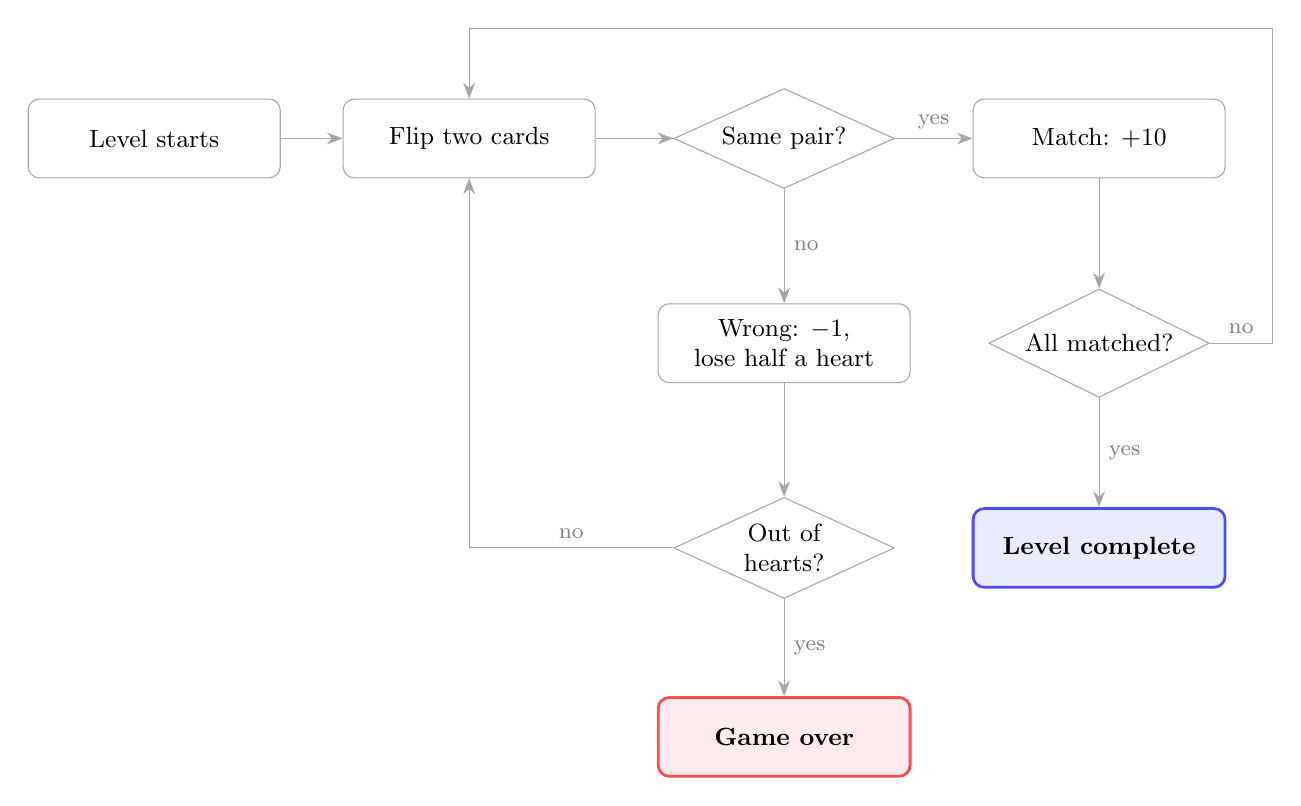
\begin{tikzpicture}[
  font=\small,
  box/.style={rectangle, rounded corners=4pt, draw=gray!70, minimum width=3.2cm, minimum height=1cm, align=center},
  dec/.style={diamond, aspect=1.8, draw=gray!70, inner sep=1pt, minimum width=2.8cm, align=center},
  good/.style={box, draw=blue!70, fill=blue!8, line width=1pt, font=\small\bfseries},
  bad/.style={box, draw=red!70, fill=red!8, line width=1pt, font=\small\bfseries},
  arr/.style={-{Stealth[length=2mm]}, draw=gray!70},
  lab/.style={font=\footnotesize, text=gray}
]
\node[box]  (start) at (0,0)     {Level starts};
\node[box]  (flip)  at (4,0)     {Flip two cards};
\node[dec]  (same)  at (8,0)     {Same pair?};
\node[box]  (match) at (12,0)    {Match: +10};
\node[box]  (wrong) at (8,-2.6)  {Wrong: $-1$,\\lose half a heart};
\node[dec]  (all)   at (12,-2.6) {All matched?};
\node[dec]  (lives) at (8,-5.2)  {Out of\\hearts?};
\node[good] (done)  at (12,-5.2) {Level complete};
\node[bad]  (over)  at (8,-7.6)  {Game over};

\draw[arr] (start) -- (flip);
\draw[arr] (flip) -- (same);
\draw[arr] (same) -- node[above, lab] {yes} (match);
\draw[arr] (same) -- node[right, lab] {no} (wrong);
\draw[arr] (match) -- (all);
\draw[arr] (all) -- node[right, lab] {yes} (done);
\draw[arr] (wrong) -- (lives);
\draw[arr] (lives) -- node[right, lab] {yes} (over);
\draw[arr] (lives.west) -- node[above, lab, pos=0.5] {no} (4,-5.2) -- (flip.south);
\draw[arr] (all.east) -- node[above, lab] {no} (14.2,-2.6) -- (14.2,1.4) -- (4,1.4) -- (flip.north);
\end{tikzpicture}
\caption{Round flow in Memory Flip: every pair matched wins the level; running out of hearts ends it.}
\end{figure}

A wrong pair sends the player back to flip again unless it emptied the last heart. A match sends them back too, until the last pair is found.

% =====================================================
\section{6. Game Mechanics}
% =====================================================
\subsection*{6.1 Flipping and matching}
Only two cards can be face up at once; extra taps are ignored until the pair is resolved. Tapping an open or already matched card does nothing. Two cards match only when they come from the same word pair, so ``Happy'' matches ``Joyful'' but not ``Calm'', even though both are positive words.

\subsection*{6.2 \hl{Point system}}
\begin{tabularx}{\textwidth}{|L|L|}
\hline
\rowcolor{headgray}\textbf{Event} & \textbf{Points} \\ \hline
Correct pair & +10 \\ \hline
Wrong pair & $-1$ and half a heart \\ \hline
\end{tabularx}

The score never falls below zero. The maximum score for a level is 10 points per pair: 60 for Level 1, 80 for Level 2, 100 for Level 3, 120 for Level 4 and 140 for Level 5.

\subsection*{6.3 \hl{Lives}, moves and time}
\begin{tabularx}{\textwidth}{|p{3cm}|L|}
\hline
\rowcolor{headgray}\textbf{Item} & \textbf{Rule} \\ \hline
Hearts & Each heart is worth two mistakes, so a wrong pair empties half a heart \\ \hline
Moves & +1 each time two cards are turned over \\ \hline
Timer & Counts up from 0:00 and stops when the level ends \\ \hline
Game over & Last heart empty: the board locks and the level ends \\ \hline
\end{tabularx}

\hl{The number of hearts grows with the board.} Even a player with perfect memory makes about 0.6 wrong guesses per pair, because some cards must be turned over before their partner has been seen. A fixed limit of three mistakes therefore made the larger levels almost impossible to win. Each level now allows roughly that unavoidable number plus a few slips (see the table in 6.4). Counting two mistakes per heart keeps the header short: Level 5 shows 6 hearts instead of 12.

\begin{figure}[h!]
\centering
\shot{10cm}{gameover.png}
\hspace{1cm}
\shot{10cm}{result.png}
\caption{Player feedback: Game Over pop-up (left) and results screen (right)}
\end{figure}

\subsection*{6.4 Levels and progression}
Each level adds two more pairs and uses harder words. Level 1 has no mistake limit so beginners can learn the rules. All levels are open from the start, so players can choose their own difficulty.

\begin{tabularx}{\textwidth}{|p{1.2cm}|L|p{1cm}|p{1cm}|p{1.8cm}|p{2.3cm}|}
\hline
\rowcolor{headgray}\textbf{Level} & \textbf{Theme} & \textbf{Pairs} & \textbf{Cards} & \textbf{Board} & \textbf{Hearts (mistakes)} \\ \hline
1 & Pictures (emoji $\leftrightarrow$ word) & 6 & 12 & 4 columns & Unlimited \\ \hline
2 & Synonyms & 8 & 16 & 4 columns & 3 (6) \\ \hline
3 & Antonyms & 10 & 20 & 5 columns & 4 (8) \\ \hline
4 & Advanced vocabulary & 12 & 24 & 6 columns & 5 (10) \\ \hline
5 & Master challenge & 14 & 28 & 6 columns & 6 (12) \\ \hline
Custom & Player-made & 2--8 & 4--16 & 4 columns & 2--4 (4--8) \\ \hline
\end{tabularx}

The board widens automatically as cards are added: 4 columns up to 16 cards, 5 up to 20, and 6 beyond that. Text on the cards shrinks on the larger boards so long words still fit.

\subsection*{6.5 Random shuffling}
The deck is shuffled every time a level starts or is replayed, so the player cannot memorise card positions between games.

\subsection*{6.6 \hl{Custom sets}}
Each entry can be up to 20 characters, and both fields must be filled. A set needs at least 2 pairs and can hold up to 8. A custom set allows one mistake per pair, rounded up to an even number, with a minimum of 4 (2 hearts).

\begin{figure}[h!]
\centering
\shot{10cm}{custom.png}
\caption{Create Custom Set screen, where players add their own word pairs}
\end{figure}

% =====================================================
\section{7. Technology and Implementation}
% =====================================================
\subsection*{7.1 \hl{From PowerApps to Lovable}}
\hl{Our midterm prototype was a PowerApps canvas app. For the final version we used {\textbf{Lovable}}, a low-code platform that builds a web app from written descriptions.} We described the screens, theme and rules in plain language, and Lovable generated the code. We then refined it with further prompts, such as reworking the mobile layout and spacing the level cards evenly.

The result is a standard web app, so it runs in any modern browser on phones and computers without installation.

\begin{tabularx}{\textwidth}{|p{4.5cm}|L|}
\hline
\rowcolor{headgray}\textbf{Part} & \textbf{Technology} \\ \hline
Low-code builder & Lovable \\ \hline
Framework & React 19 with TanStack Start \\ \hline
Language & TypeScript \\ \hline
Styling and animation & Tailwind CSS (card flip done with CSS 3D transforms) \\ \hline
Build and local server & Vite \\ \hline
Version control & Git, synced with Lovable \\ \hline
\end{tabularx}

\subsection*{7.2 Screens and components}
The game keeps the same five screens as the PowerApps prototype, with the same names: \textbf{scrMenu}, \textbf{scrLevelSelect}, the \textbf{Game} screen, \textbf{scrCreateSet} and \textbf{scrGameOver}. One state value records the current screen, and changing it swaps the screen with a short fade-and-slide animation.

All levels share one Game screen. When a level is chosen, the game loads that level's word pairs and builds the board from them. New levels can be added by adding a list of word pairs, with no new screen needed.

\subsection*{7.3 Game data}
Each level is stored as a name, an icon, a short description, its number of allowed mistakes and a list of word pairs. The data for the five built-in levels holds 50 word pairs in total. Custom pairs are kept in the app's state while it is open.

\subsection*{7.4 Game state}
React state tracks the shuffled deck, the cards currently face up, the matched pairs, score, moves, time and mistakes. A timer adds one second each second and stops when the level is won or lost.

\subsection*{7.5 Game logic}
\begin{itemize}
  \item \textbf{Deck building:} each word pair becomes two cards with the same pair number, then the deck is shuffled.
  \item \textbf{Match check:} when two cards are open, the game compares their pair numbers.
  \item \textbf{Scoring:} a match adds 10 points; a mismatch removes 1 point and adds a mistake.
  \item \textbf{Win and lose:} the level is won when every pair is matched and lost when its hearts run out.
\end{itemize}

The matching rule in code:
\begin{lstlisting}
if (deck[x].pair === deck[y].pair) {
  score = score + 10;              // match: cards stay open
} else {
  score = Math.max(0, score - 1);  // mismatch: cards flip back
  mistakes = mistakes + 1;         // empties half a heart
}
// Level 1 has no limit; other levels end when the hearts run out
const lost = level.lives !== undefined && mistakes >= level.lives;
\end{lstlisting}

% =====================================================
\section{8. Prototype Overview}
% =====================================================
\subsection*{8.1 Midterm prototype (PowerApps)}
The midterm prototype was a PowerApps canvas app. It had the menu, level select and game-over screens, two levels, and the basic flip-and-match loop.

\subsection*{8.2 \hl{Improvements in the final version (Lovable web app)}}
\begin{itemize}
  \item \hl{Five built-in levels with 50 word pairs, from picture words to master vocabulary}
  \item \hl{Hearts that grow with the level (half a heart per mistake) and a Game Over screen with Try Again}
  \item \hl{Live score, move counter and timer in the game header}
  \item \hl{Working Custom Set builder for 2 to 8 player-made pairs}
  \item \hl{3D card-flip animation, match highlight and pop-up feedback}
  \item \hl{Board that resizes from 4 to 6 columns for larger levels}
  \item \hl{Mobile-first layout that also works on tablets and computers}
\end{itemize}

\subsection*{8.3 Features under development}
\begin{itemize}
  \item Saving custom sets and best scores in the browser, so they remain after the page is closed
  \item Unlocking levels in order, with a star rating based on mistakes
\end{itemize}

\subsection*{8.4 \hl{Final presentation demonstration}}
\begin{enumerate}
  \item The menu screen and the level list with all five levels.
  \item Level 1: matching a picture with its word, with no mistake limit.
  \item Level 2: a wrong pair flipping back ($-1$ point, half a heart lost).
  \item Finishing a level, then the Level Complete pop-up and the results screen.
  \item Running out of hearts to show the Game Over pop-up.
  \item Creating a custom set of class vocabulary and playing it.
\end{enumerate}

% =====================================================
\section{9. Future Development}
% =====================================================
Beyond the features under development, we plan to add:
\begin{itemize}
  \item \textbf{Hints:} briefly reveal one matching card, at a points cost.
  \item \textbf{Sound effects:} for flips, matches and mistakes, with a mute setting.
  \item \textbf{Word meanings:} show a short definition when a pair is matched, so players learn what new words mean.
  \item \textbf{Shareable word sets:} let a teacher create a set and share it with a class through a link.
  \item \textbf{Two-player mode:} players take turns on the same device and compare pairs found.
  \item \textbf{Usability testing:} with around ten classmates, to check difficulty and whether players learn new words.
\end{itemize}

% =====================================================
\section{10. Conclusion}
% =====================================================
Memory Flip turns the classic memory card game into a vocabulary-learning game. Its central idea is that each pair is a word and its meaning, so players must remember positions and know the words at the same time.

\hl{Our midterm PowerApps prototype proved the basic flip-and-match loop. For the final version we rebuilt the game with the low-code tool Lovable as a responsive web app.} It now has five levels, hearts that grow with the difficulty, live scoring, animated feedback and a custom word-set builder.

Our next steps are to save progress in the browser, add level unlocking and star ratings, and test the game with real players.

\end{document}
